\vspace{-1pt}
\section{Community Detection Results} \label{cd}
\begin{table*}
\begin{tabular}{ |p{3cm}||p{3cm}|p{3cm}||p{3cm}|p{3cm}|  }
 \hline
 \multicolumn{1}{|c||}{}&\multicolumn{2}{c||}{Gamergate Dataset}&\multicolumn{2}{c|}{U.S. Presidential Election Dataset}\\
 \hline
Method & F1 Score &Jaccard&F1 Score &Jaccard\\
 \hline
 CESNA   & 0.343    & 0.211&0.253 &0.149\\
 Modularity&  0.434   & 0.282 &0.753 &  0.604\\
 CLAN & \textbf{0.478}&\textbf{0.318} & \textbf{0.787}
&\textbf{0.649}\\
 \hline
\end{tabular}
\caption{The quantitative results obtained from calculating the F1 and Jaccard similarity scores with regards to the ground truth labels for each of the methods.}
\label{resulttable}
\end{table*}
\begin{table*}
\centering
\begin{tabular}{ |m{4.5cm}||m{4.5cm}||m{4.5cm}|  }
\hline \multicolumn{1}{|c}{}&\multicolumn{1}{c}{Unlabeled Users}&\multicolumn{1}{c|}{}\\
 \hline
 \multicolumn{1}{|c||}{Method}&\multicolumn{1}{c||}{Gamergate Dataset}&\multicolumn{1}{c|}{U.S. Presidential Election Dataset}\\
 %FM:  No need to say "percentage of" when you have the percents.
% FM: (Just minimized the table a little) Method & Unlabeled Users&Unlabeled Users\\
%NM:Fixed!
 \hline
 CESNA   &   69\%  &95\% \\
 Modularity& 21\%   &  20\%\\
 CLAN & 0\%&0\%\\
 \hline
\end{tabular}
\caption{Percentage of unlabeled users in each of the methods.}
\label{percentage} % (Add the label here)
\end{table*}
\begin{figure*}[!b]
  \centering
  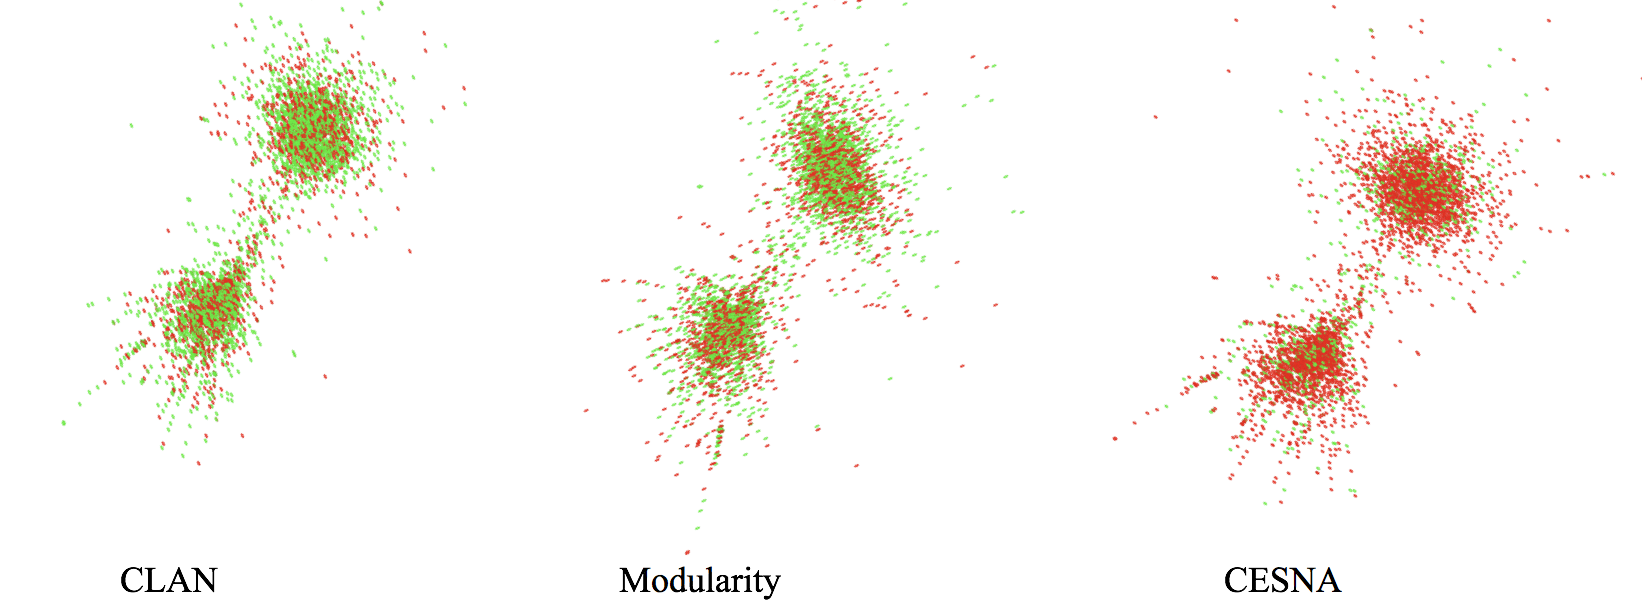
\includegraphics[width=\textwidth]{big_non_axis.png}
  \caption{Networks colored by agreement with the ground truth labels for three methods for the Gamergate dataset.}
  \label{agreement}
\end{figure*}
 
\begin{table*}
\centering
\begin{tabular}{ |p{6.5cm}||p{2.5cm}|p{2.5cm}|p{2.5cm}|p{2.5cm}|  }
 \hline
 Gamergate Tweet&CESNA Label&Modularity Label&CLAN Label&Ground Truth Label\\
 \hline
``\#gamergate is like a particularly lame version of pakistani twitter political flame wars like ridiculously lame"&N/A&N/A&Anti Gamergate &Anti Gamergate\\[0.5pt]
 \hline
 ``\#gamergate is brutally put in its place by a journalist``&N/A&N/A&Anti Gamergate &Anti Gamergate\\[0.5pt]
 \hline
 ``\#gamergate \#done i suspect the \#ottawashooting has more in common with \#montrealmassacre \#columbine \#gamergate than it does with \#islam``&N/A&N/A&Anti Gamergate &Anti Gamergate\\[0.5pt]
  \hline
%  ``\#gamergate \#notyourshield a victory for \#gamergate or against yellow journalism \#notyourshield \#gamergate. gamers are like honey badgers you do not out-fight a honey badger  \#notyourshield \#gamergate may you receive a billion retweets. if \#notyourshield was recognized by the media ppl like joss whedon would have to admit they were wrong about \#gamergate  \#gamergate. read the calm demeanor of the gamergate person versus the fanaticism of the anti-gamergate ... where do you think gawker got their tactics from the \#gop and fox news practically taught them how to suppress \#gamergate``&N/A&N/A&Gamergate Supporter&Gamergate Supporter\\[0.5pt]
%   \hline
 ``\#gamergate i support \#gamergate and \#notyourshield i stand against harassment threats and doxxing no matter who or why``&N/A&N/A&Gamergate Supporter&Gamergate Supporter\\[0.5pt]
 \hline
 ``\#gamergate \#extralife2014 only two more days until our stream starts are you hyped we sure are current score to beat 100. I just supported \#gamergate extra life charity``&N/A&Gamergate Supporter&Gamergate Supporter&Gamergate Supporter\\[0.5pt]
 \hline
\end{tabular}
\caption{Sample Gamergate users with their corresponding tweets and labels assigned to each user by the three methods. ``N/A'' means that the method failed to classify the user.}
\label{gamergateexamples}
\end{table*}
\begin{table*}[!b]
\centering
\begin{tabular}{ |p{6.5cm}||p{2.5cm}|p{2.5cm}|p{2.5cm}|p{2.5cm}|  }
 \hline
 2016 U.S. Presidential Election Tweet & CESNA Label & Modularity Label & CLAN Label&Ground Truth Label\\
 \hline
``Trump wants to ban Muslim immigrants like my parents. I wrote a piece for telling him to go fuck himself.``&N/A &N/A &Democrat &Democrat\\[0.5pt]
 \hline
 ``Frauds at NY Times coverup Hillary's serious crimes...but try to make Trump into a criminal for LEGAL tax reduction strategy. WOW.``&N/A&Republican&Republican&Republican\\[0.5pt]
 \hline
 ``Fox News Host Makes Hillary Supporter Admit That Clinton Foundation Is A Huge Scam.``&Democrat&Republican&Republican&Republican\\[0.5pt]
  \hline
\end{tabular}
\caption{Sample 2016 U.S. Presidential Election users with their corresponding tweets and labels assigned by the three methods.}
\label{electionexample}
\end{table*}
Our goal is to report quantitative and qualitative results obtained through different experimentation in this paper. Hence, we use different visualizations and examples from datasets in hand, in addition to our numerical results to give the reader a better intuition of how our method, CLAN, performs compared to the existing state of the art. %FM: We need to rewrite this.
%NM: Rewrote this part and got rid of the superiority portion
\subsection{Evaluation Metrics}
For evaluation purposes, the F1 and Jaccard similarity scores are calculated for each of the datasets with respect to the ground truth labels. These scores are the average values of the total communities found in each of the datasets. 
%The ground truth labels and their collection procedure for each of the datasets are discussed in detail under the datasets section.%
% FM: Didn't we already do this?
%NM: True and I commented it out! Fixed.

\subsubsection{Quantitative Results} In this section, we would report quantitative and numerical results from our experiments. We will first report the scores for the F1 and Jaccard similarity scores between the ground truth labels and three different methods. We will show that CLAN outperforms other methods in terms of F1 and Jaccard similarity scores for both of the datasets. %FM: Isn't this redundant?
%NM: Fixed it!
Table \ref{resulttable} contains results for the F1 and Jaccard similarity scores obtained from comparisons done between the ground truth labels and labels obtained by applying each of the methods on the two datasets on hand.

In addition to reporting the F1 and Jaccard score results from the ground truth comparisons, we conducted another experiment in which we report the results indicating the number of the users that were labeled by each of the methods. % FM: we need to rewrite this.
%fixed
These numbers show the number of users that the method has excluded by not labeling them. This exclusion shows the bias of the method towards those users. Therefore, the more unlabeled users a method has the more susceptible to bias it is. In Table~\ref{percentage}, %FM: reference it like this. 
%NM:Fixed!
we reported the percentage of the users who were left unlabeled or put in insignificant communities in each of the methods from the two datasets. These results confirm the fact that our method, CLAN, has mitigated the bias towards the introverted users by incorporating them into the significant communities which would not be excluded from various down stream data analysis tasks.

The two sets of results reported in Tables \ref{resulttable} and \ref{percentage} confirm that not only is our method able to achieve superior predictive accuracy but also mitigate bias against introverted users by assigning them labels preventing them from exclusion.
%\FloatBarrier
\subsubsection{Qualitative Results} Besides the numerical results reported in the previous subsection, we want to further our analysis by showing some visualized results and real examples drawn from our datasets to further prove our results from the previous subsection. We will start our qualitative results by showing a visualization of the retweet network in the Gamergate dataset in the three methods discussed in this paper. Each node in these graphs represent a user and the nodes are color coded based on their agreement with the ground truth labels. The green nodes represent agreement between the label that was assigned to that particular user obtained from the method used and the ground truth label, and the red node represent disagreement between the two labels associated to that node. Therefore, more green nodes in a graph represent the degree of agreement of that method with the ground truth label and generally its superiority in terms of agreement with the ground truth compared to the other methods. The results of these visualizations are shown in Figure \ref{agreement}.
In addition to disagreement, the red nodes may also represent the fact that a method has low recall value and that many users were assigned no labels while the ground truth has assigned it a label. This of course is a sort of disagreement between the labels, so the nodes are colored as red. As expected, CESNA would have many red nodes as this method tends to have a very low recall value and as shown in Table \ref{percentage}, this method has a high tendency to exclude many users by not assigning them a label. Therefore, it suffers from low agreement with the ground truth and as expected highly covered by red nodes. This also confirms the existence of bias towards these red users who suffered from CESNA's low recall issue. The result associated to this method is shown on the far right side of Figure \ref{agreement}. As we move to the next method in the middle of Figure \ref{agreement}, we see less red nodes. This is because using modularity value has a higher recall and generally more agreement with the ground truth, but one can still spot many red users in this method. Moving on to the last graph on the far left side of Figure \ref{agreement}, we can see the graph associated to CLAN. Due to CLAN's use of node attributes in addition to the network attributes, it is able to obtain higher agreement with the ground truth and therefore less red nodes compared to the previous method. CLAN was able to address many red nodes in the top portion as well as the bottom portion of the graph compared to the modularity method.
\begin{figure*}
  \centering
  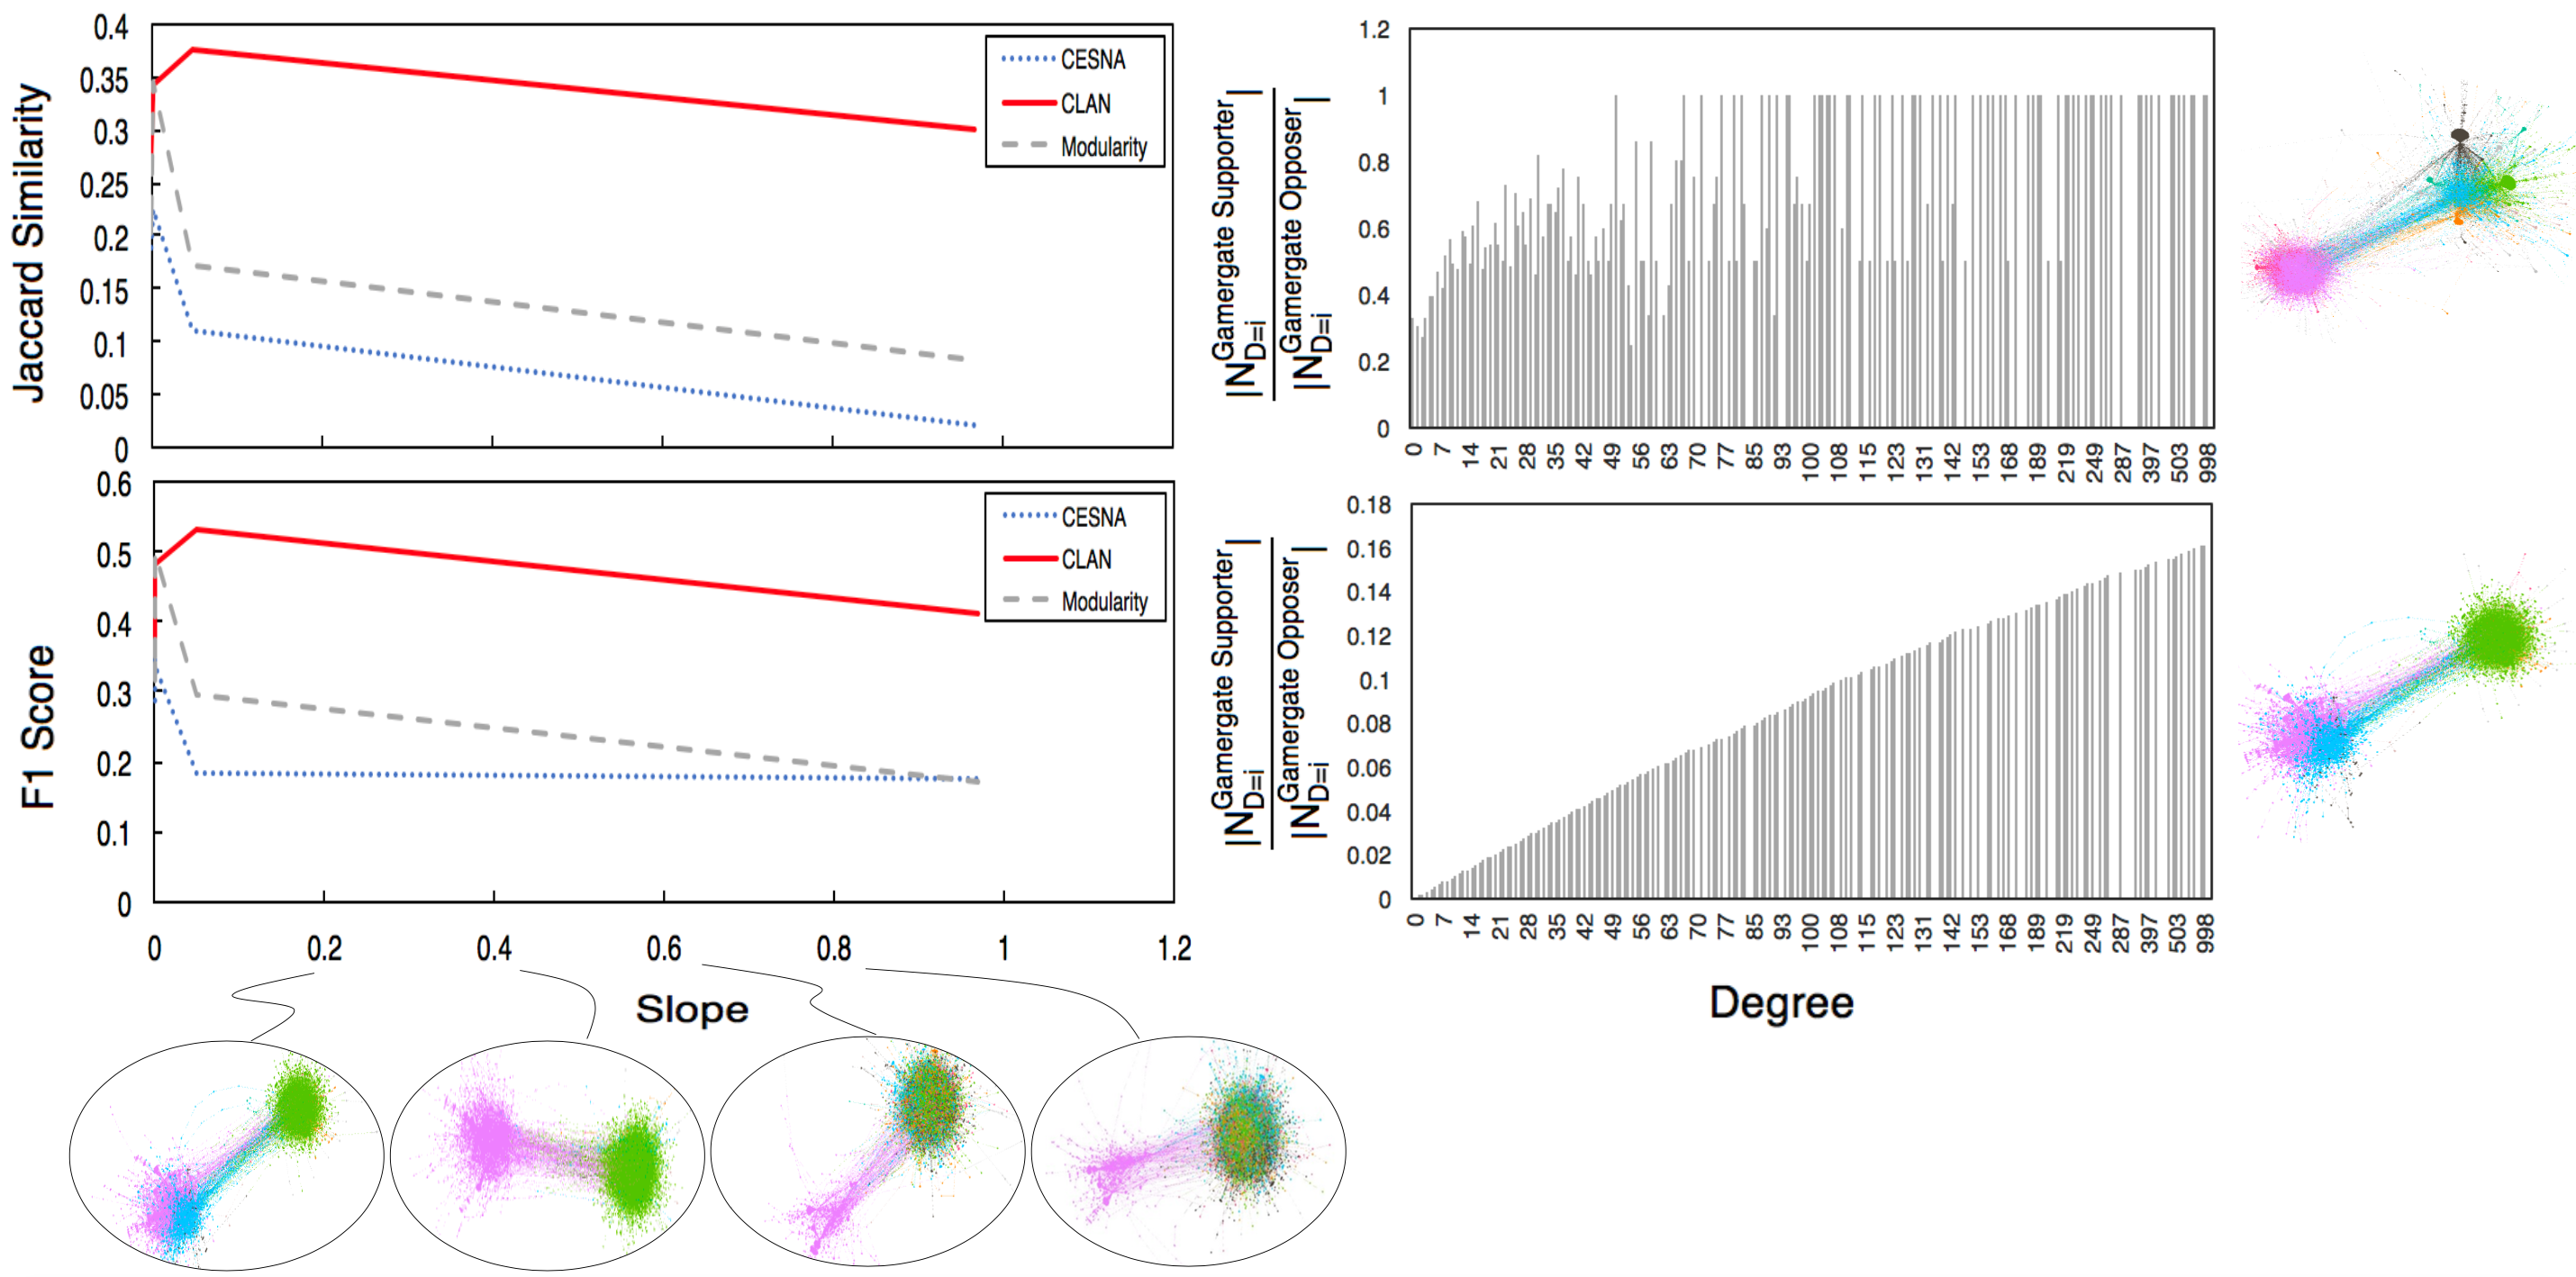
\includegraphics[width=\textwidth]{nex.png}
  \caption{Synthetic distributions with their corresponding network and obtained results for the Gamergate dataset.}
  \label{synthetic1}
\end{figure*}
In addition to the agreement graphs shown in Figure \ref{agreement}, we provided two sets of tables, Table \ref{gamergateexamples} and \ref{electionexample}, in which some examples from each of the datasets are provided where it shows how each of the methods labeled a particular user with sets of tweets they tweeted. The ground truth labels are also listed for comparison purposes. Table \ref{gamergateexamples} contains the results from the Gamergate dataset, while Table \ref{electionexample} contains the results for the 2016 presidential election dataset. These examples also highlight the fact that the baseline approaches are suffering from the type of bias that roots from exclusion of users by not assigning them any labels or putting them into insignificant communities that would be excluded.

The qualitative results reported in this subsection also confirm the fact that the baseline methods have low agreement with the ground truth labels and suffer from bias towards low-degree and some users who are excluded from being labeled. The results from this and previous subsection also show the superiority of our method in terms of addressing these issues through various examples provided.
